%
% watts_engine.tex -- template for standalon tikz images
%
% (c) 2021 Prof Dr Andreas Müller, OST Ostschweizer Fachhochschule
%
\documentclass[tikz]{standalone}
\usepackage{amsmath}
\usepackage{times}
\usepackage{txfonts}
\usepackage{pgfplots}
\usepackage{csvsimple}
\usetikzlibrary{arrows,intersections,math,calc}
\definecolor{darkred}{rgb}{0.8,0,0}
\definecolor{darkgreen}{rgb}{0,0.6,0}
\begin{document}
\def\skala{1}
\begin{tikzpicture}[>=latex,thick,scale=\skala]

    % Insert image
    \node[inner sep=0, anchor=south west] (img) at (0,0) {
        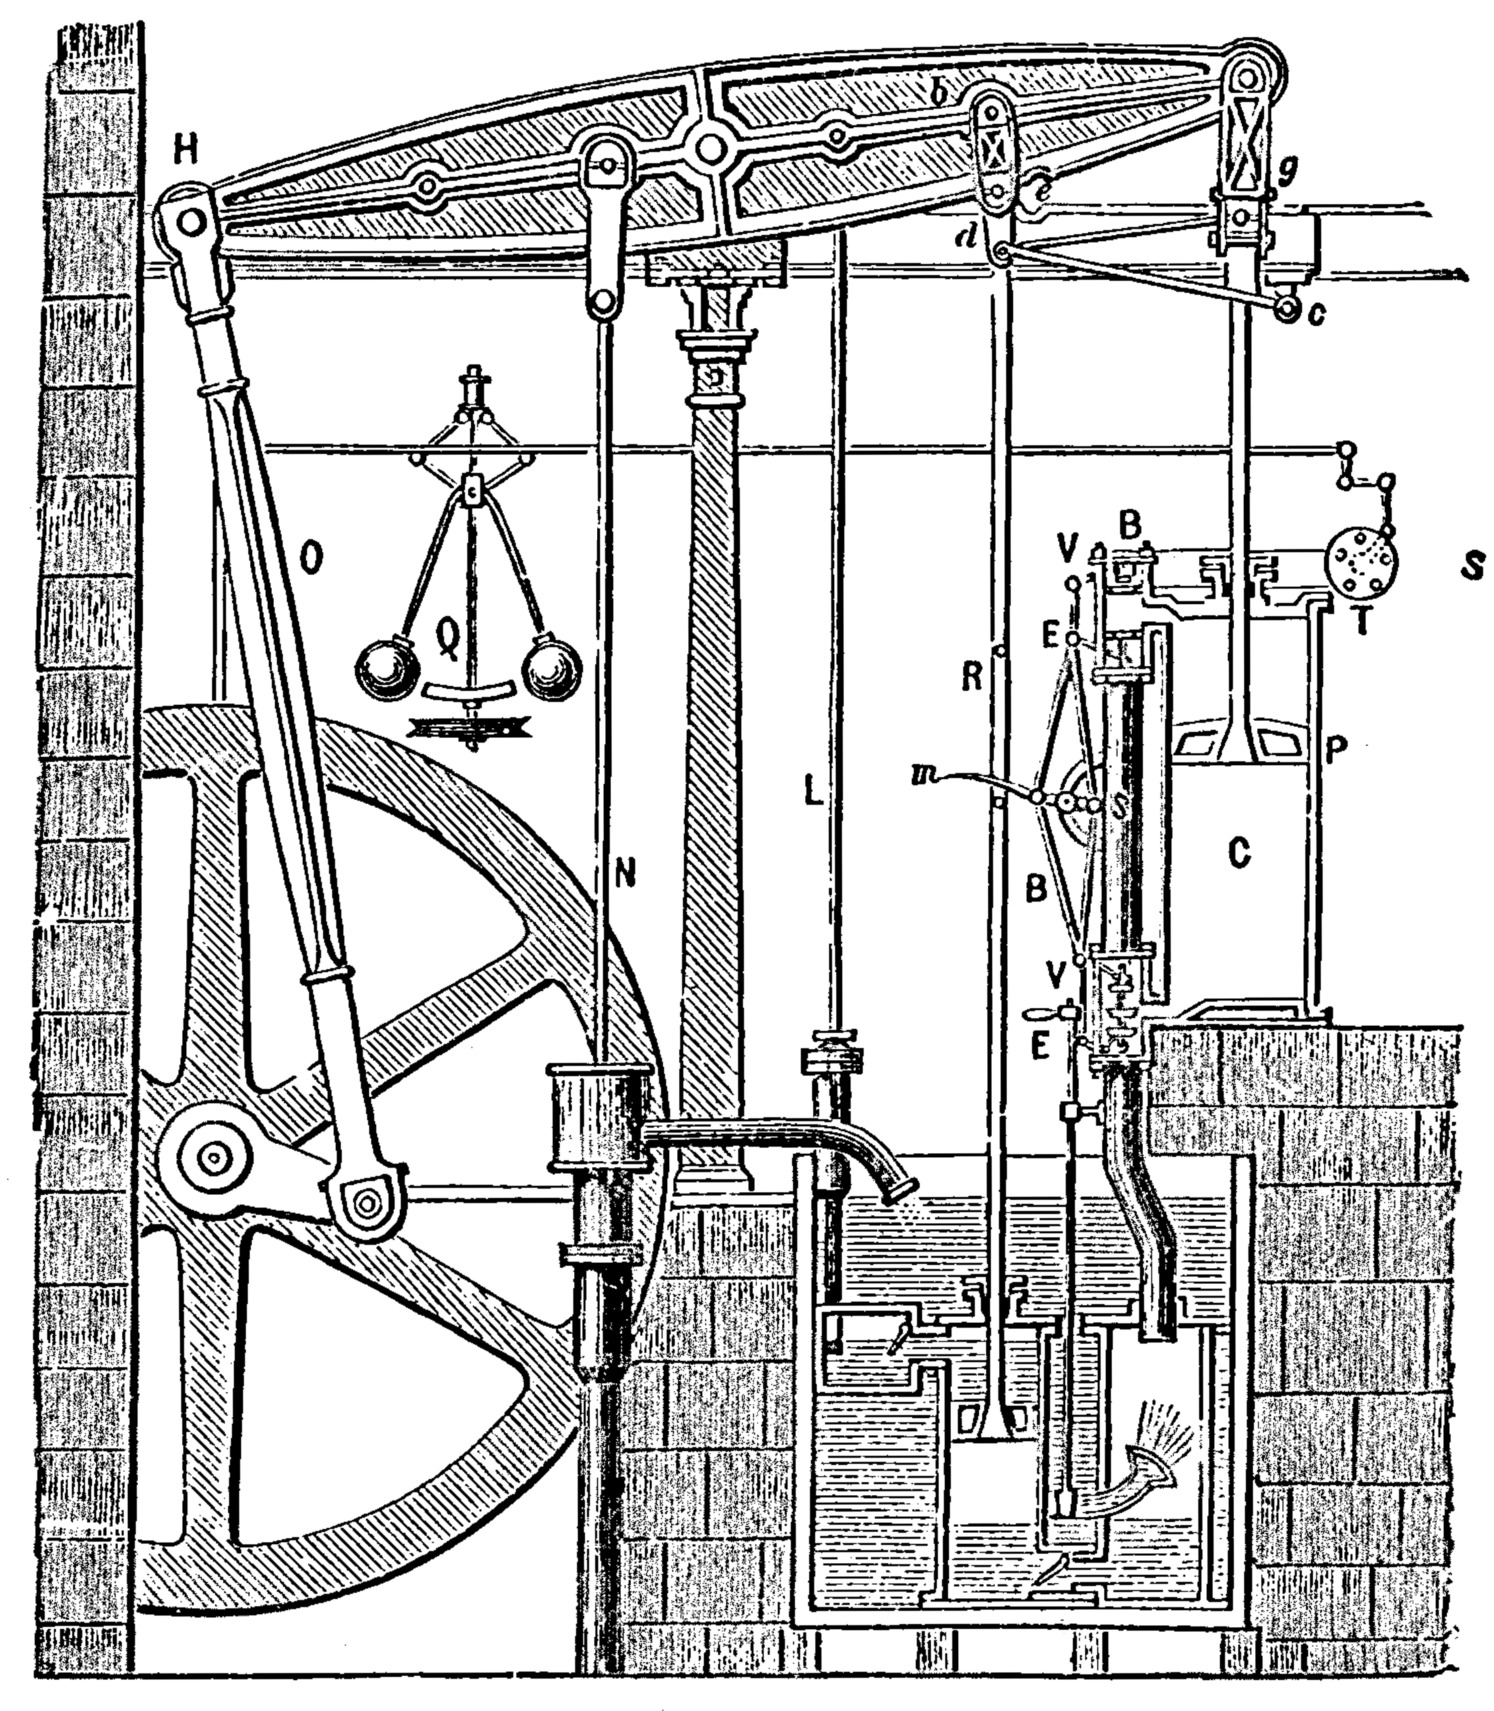
\includegraphics[width=0.9\textwidth]{watts_engine-small.jpeg}
        % 
\includegraphics[width=0.9\textwidth, trim=3cm 2cm 3cm 10cm, clip]{papers/geradlinig/figures/watts_engine.jpeg}
    };

    % Normalized coordinate system over the image
    \begin{scope}[x={(img.south east)}, y={(img.north west)}]
        % % Grid (0 to 10 in both directions)
        % \draw[step=0.1, gray!30] (0,0) grid (1,1);
        % \draw[step=0.2, gray!60] (0,0) grid (1,1);

        % % Axes
        % \draw[->, very thick] (0,0) -- (1.05,0) node[right=2pt] {$x$};
        % \draw[->, very thick] (0,0) -- (0,1.05) node[above=2pt] {$y$};
        
        % % Tick marks and integer labels
        % \foreach \i in {0,1,...,10} {
        %     \draw[black] (\i/10,0) -- (\i/10,-0.01);
        %     \draw[black] (0,\i/10) -- (-0.01,\i/10);
        %     \node[below] at (\i/10,0) {\small \i};
        %     \node[left] at (0,\i/10) {\small \i};
        %     }
            
        %     % Arrow decoration style for drawing arrows along a path
        %     \tikzset{arrow along path/.style args={#1 and #2}{
        %         decoration={markings, mark=between positions #1 and 0.95 step #2 with {\arrow[scale=1.0]{>}}},
        %         postaction={decorate}
        %         }}
            
            % % Individual drawings for picture
            \coordinate (A) at (0.475,0.915);
            \coordinate (B) at (0.67,0.934);
            \coordinate (C) at (0.83,0.95);
            \coordinate (D) at (0.67,0.85);
            \coordinate (E) at (0.83,0.87);
            \coordinate (F) at (0.86,0.82);
            
            \definecolor{jointblue}{RGB}{102,204,255}
            \definecolor{jointgreen}{RGB}{102,153,102}
            \definecolor{jointyellow}{RGB}{255,204,102}
    
            \draw[jointblue,   line width=3pt, draw opacity=0.8] (A) -- (C);
            \draw[jointgreen,  line width=3pt, draw opacity=0.8] (B) -- (D);
            \draw[jointgreen,  line width=3pt, draw opacity=0.8] (C) -- (E);
            \draw[jointyellow, line width=3pt, draw opacity=0.8] (E) -- (D);
            \draw[jointyellow, line width=3pt, draw opacity=0.8] (D) -- (F);
            
            \fill (A) circle[radius=4pt];
            \fill (B) circle[radius=4pt];
            \fill (C) circle[radius=4pt];
            \fill (D) circle[radius=4pt];
            \fill (E) circle[radius=4pt];
            \fill (F) circle[radius=4pt];

            \end{scope}

\end{tikzpicture}
\end{document}

